% 作者:海南大学2015级计算机 Dxr

\documentclass[article,12pt,a4paper,onesides,UTF8]{ctexart} % 期刊类型,全局默认小四字体,a4纸张,单面打印,调用ctex宏包
% 等于\documentclass[UTF8]{article} 
\usepackage{ctex}
\usepackage[top=2.54cm,bottom=2.54cm,left=3.17cm,right=3.17cm]{geometry} % 调用geometry宏包设置页边距
\usepackage{pdfpages} % 调用PDF宏包
\usepackage{fancyhdr} % 页眉页脚
\usepackage{graphicx} % 调用图片包
\usepackage{caption} % 调用设置图片格式包
\usepackage{enumerate} % 调用生成列表包 (1)海大四级标题
\usepackage{enumitem} % 修改列表包
\usepackage{setspace} % 调整行间距
\usepackage{titletoc}
\usepackage{titlesec} % 设置标题样式
\usepackage[namelimits]{amsmath} %数学公式
\usepackage{amssymb} % 数学公式
\usepackage{amsfonts} % 数学字体
\usepackage{mathrsfs} % 数学花体
\usepackage{tabularx} % 表格
\usepackage{booktabs} % 调整表格
\usepackage{longtable} % 表格跨页,有问题
\usepackage[ruled,linesnumbered]{algorithm2e} % 算法
\usepackage[super,square,compress,sort]{natbib}% 参考文献样式
% \usepackage{setspace}%调整行间距
% \usepackage{fontspec} % 字体宏包,和PDF冲突……
%% 全局设置
% 设置字体
\newcommand{\sanhao}{\fontsize{16pt}{\baselineskip}\selectfont} \newcommand{\xiaosan}{\fontsize{15pt}{\baselineskip}\selectfont} \newcommand{\sihao}{\fontsize{14pt}{\baselineskip}\selectfont} \newcommand{\xiaosi}{\fontsize{12pt}{\baselineskip}\selectfont} \newcommand{\wuhao}{\fontsize{10.5pt}{\baselineskip}\selectfont}
% 设置字体

%全行间距
\renewcommand{\baselinestretch}{1.5}  % 调整全局行距为1.5

% 各级标题调整
\CTEXsetup[format={\sanhao\bfseries}]{section} % ctex中第一章标题默认居中,但是海大的要求顶格,重置为居左(\bfseries)。三号\粗体
\CTEXsetup[format={\sihao\bfseries}]{subsection} % 二级标题四号加粗
\CTEXsetup[format={\xiaosi\bfseries}]{subsubsection} % 三级标题小四加粗
\setenumerate[enumerate]{fullwidth,itemindent=2em,listparindent=2em,label=(\arabic*)} % 设置四级标题,学校四级标题样式为(1)\setlist
% itemindent:条目的缩进距离,listparindent 条目下面段

%% 另外一种设置方式
% \titleformat{\section}{\sanhao\bfseries}{\arabic{section} }{0.5em}{} % 设置标签与标题内容之间以一个字(0.5em)的宽度为间隔

% \titleformat{\subsection}{\sihao\bfseries}{ \thesection.\arabic{subsection}}{0.5em}{} % 设置标签与标题内容之间以一个字(0.5em)的宽度为间隔

%\titleformat{\subsubsection}{\xiaosi\bfseries}{ \thesection.\arabic{subsection}.\arabic{subsubsection}}{0.5em}{} % 设置标签与标题内容之间以一个字(0.5em)的宽度为间隔


%页眉页脚
\pagestyle{fancy} % 设置页眉
\renewcommand{\headrulewidth}{0.4pt} % 页眉线宽度0.4pt,设0可去掉页眉线(默认为0)
%% 全局设置

% 目录样式
\lhead{}
\rhead{}
\cfoot{}

\titlecontents{section}[5mm] % 标题位置,左间距5毫米
{\zihao{-4}} % 字号小四
{\filleft\contentslabel{1em}} % 标题标志 (设置标题标志的格式,如序号格式、序号宽度、序号与标题内容之间的间距等,不可空置)
{\hspace*{-1em}} %保证摘要等对齐  contentslabel 的距离与此处的hspace大小相等,正负相反,即可对齐
{\titlerule*{.}\contentspage} % 指引线与页码 (设置标题与页码之间的指引线样式以及页码的格式,该参数如果空置,标题将无指引线和页码)

\titlecontents{subsection}[9mm]
{\xiaosi} % 字号小四
{\contentslabel{2em}}
{\hspace*{-2em}}
{\titlerule*{.}\contentspage}

\titlecontents{subsubsection}[11mm]
{\xiaosi} % 字号小四
{\contentslabel{2.5em}}
{\hspace*{-2.5em}}
{\titlerule*{.}\contentspage}
% 目录样式

% 图片设置
\graphicspath{{graphics/}}%设置图片路径为当前路径下的graphics文件夹
\renewcommand{\thefigure}{\wuhao{\thesection-\arabic{figure}}}
% 图片命名默认样式是 图1:,按照论文要求格式改为 图1-1(无冒号)
\captionsetup{labelformat=default,labelsep=space} % 去除冒号
% 图片设置


% 内容
\begin{document}
%封面
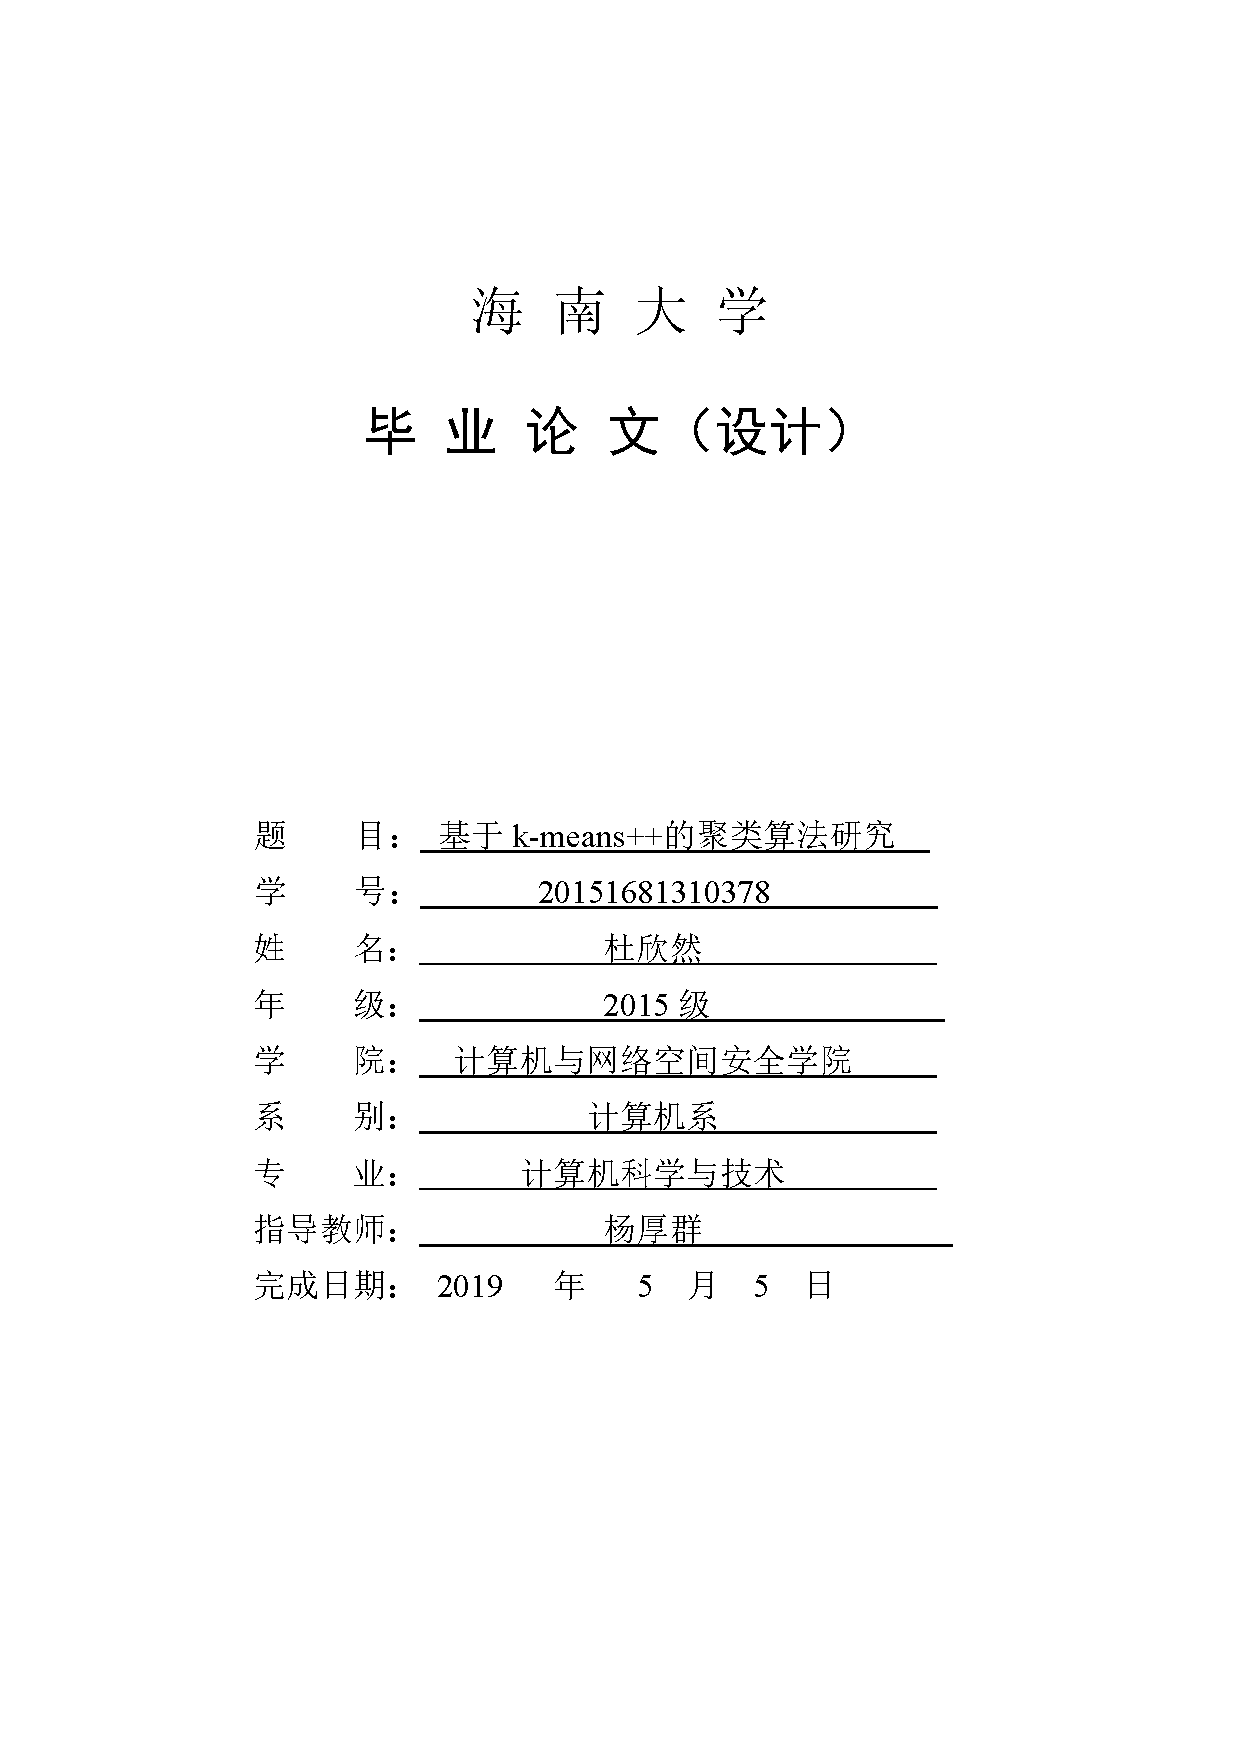
\includepdf{contents/cover.pdf} % 调用学校已经排版好的封面
%封面

\chead{\zihao{5}基于k-means++的聚类算法研究}


% 中英文摘要
% !Mode:: "TeX:UTF-8"
\newpage
\cfoot{}
% \addcontentsline{toc}{section}{摘\ \ 要}%加入目录
\centerline{\zihao{3}{摘\ \ \ \ 要}} % 三号,加粗,居中

\vspace {12pt}  %空1行

随着计算机应用日趋广泛和深入,网络安全问题也更加复杂和突出,它不仅仅关系到我们个人的隐私,更关系到商业利益乃至国家安全。现有的各种安全技术可以保证网路环境一定的安全性,但由于攻击手段层出不穷,现有安全技术也无法保证绝对安全。如何监控网络攻击并做出相应的防御已成为当今网络安全需要解决的重要问题。
% \par
数据是网络时代的产物,传统的基于数据挖掘的入侵检测模型完全依赖于数据挖掘算法对已标记数据集中数据样本的学习。数据样本标记的正确性和纯度对于构建有效的入侵检测系统至关重要。但网络中的数据量巨大,想要得到纯净的样本数据代价极大。因此寻找一种对数据集要求不那么高的入侵检测方法至关重要。

基于以上背景,本文基于聚类技术进行入侵检测研究。本实验是在Windows平台,采用Anaconda集成环境,对KDD99数据集进行处理分析,在未知数据样本类别的情况下,通过计算样本彼此间的距离来估计样本所属类别,最终得出聚类结果。



\vspace {12pt}

\noindent{\textbf{[关键词]:} % 临时取消行缩进,加粗
数据;网络安全;聚类
% !Mode:: "TeX:UTF-8"
\newpage
\cfoot{}
% \addcontentsline{toc}{section}{摘\ \ 要}%加入目录
\centerline{\zihao{3}{Abstract}}
\vspace {12pt}

 With the increasing and deepening of computer applications, network security issues are more complex and prominent. It is not only related to our personal privacy, but also to commercial interests and even national security. The existing security technologies can guarantee a certain security of the network environment, but because of the endless stream of attacks, existing security technologies cannot guarantee absolute security. how to monitor network attacks and make corresponding defenses has become an important issue that needs to be solved in today's network security.
 
 Data is a product of the network age. The traditional data mining-based intrusion detection model relies entirely on data mining algorithms for learning data samples in tagged data sets. The correctness and purity of the data sample markers is critical to building an effective intrusion detection system. But the amount of data in the network is huge, and it takes a lot of money to get pure sample data. Therefore, it is important to find an intrusion detection method that requires less high data sets.
 
 Based on the above background, this paper conducts intrusion detection research based on clustering technology. This experiment is based on the Windows platform, using the Anaconda integrated environment to process and analyze the KDD99 dataset. In the case of unknown data sample categories, the sample is classified by calculating the distance between the samples, and finally the clustering result is obtained.

\vspace {12pt}
\noindent\textbf{[Key Words]:}
data;network security;clustering

% 中英文摘要

% 目录
\renewcommand{\contentsname}{\zihao{3}\centerline{目\quad\quad\quad\quad 录} }  % 修改默认样式,目录两字用三号字体,居中
\tableofcontents   % 插入目录
% 目录

% 正文

% 页眉页脚重新设置
\newpage
\rhead{} % ctex默认第一章标题在页眉右边,置空则取消
\cfoot{\zihao{-5}\thepage} % 页脚显示页码,采用小五字体
\pagenumbering{arabic}   %页码使用阿拉伯数字
\setcounter{page}{1} % 将当前页码置为1

% 论文各个章节
% !Mode:: "TeX:UTF-8"
\section{绪论}

\subsection{选题的背景及意义}
\subsubsection{选题的背景}
由于计算机技术的不断更新,人们已经完全进入了互联网时代。与此同时,网络安全问题日益严重。互联网的广泛开放和移动支付的普及使得一些重要领域受到了越来越多的入侵攻击。网络安全不仅是一个技术问题,而且已成为全球主要的信息安全问题。

最大的勒索病毒比特币勒索软件在2018年袭击了世界,造成了无法估量的损失。尽管网络安全问题得到广泛的关注,但此类事件并未减少。因此,构建数据分析模型使安全人员能够及时检测入侵十分重要,性能好的数据分析模型不仅预测准确,还能节省预测的时间成本。

\subsubsection{选题的意义}
目前世界上入对侵检测的研究涉及众多学科,如统计学、数据挖掘、机器学习等。为了获得更好的入侵特征,本课题基于聚类分析,从网络信息安全领域的先验知识入手,提取那些反映出网络异常行为的特征,然后使用恰当的算法对处理后的数据进行挖掘。

本课题的研究重点是基于网络的无监督异常检测系统的数据分析方法。由于入侵检测要分析的数据量巨大,数据特征复杂、维度较高,因此在聚类分析前要对数据进行大量处理,以便于观察和分析聚类结果。

\subsection{国内外发展状况及其研究方向}

入侵检测系统,简称IDS(Intrusion Detection System),是网络空间安全中的一个重要问题。 它是一个实时监控网络或网络内部的系统。 一旦发现攻击尝试或攻击,IDS将发出警告并提示以确保网络安全。 由于传统防火墙大多使用静态防御并且缺乏实时警告,因此它们也无法攻击深度攻击。而 IDS可以实时响应入侵。

现如今,国外的一些研究机构对入侵检测的研究水平较高,普渡大学、加州大学的Davis分校等在此领域处于国际领先高度。国外的一些知名厂商如Cisco等对于此的研究也很深入。对于IDS的研究国内起步的较晚,但发展迅速,许多国内厂商已经转向入侵检测领域,并且还推出了自己的网络安全产品,如中科网络的“天眼”入侵检测系统,启明星辰的SkyBell和绿盟网络入侵检测。 然而,由于当前入侵检测技术中的各种缺陷,并且各种类型的攻击不断更新,误报率和误报率都很高。 因此,需要进一步提高入侵检测的准确性。就目前而言,模式匹配技术仍然是大多数成熟商家用作IDS的主要技术。

\subsection{本课题的研究概况}
\subsubsection{研究内容}
\subsubsection{研究重点及难点}


\subsection{论文的结构及内容安排}
第一章为绪论。介绍了课题的背景和本课题重要性,除此之外,基于国内外对网络入侵检测的研究现状,简要介绍了研究的内容、难点以及本课题的主要工作。

第二章为本课题使用的相关技术的概述。介绍了开发环境、开发语言以及配套技术,为本课题做准备工作。

第三章为数据集预处理。介绍了分析数据集的方法并通过特征工程执行特征提取和特征降维。

第四章为聚类算法设计。本章分析k-means算法并对其进行优化以实现更好的聚类结果。

第五章为总结。指出在数据预处理中忽视的细节和需要进行改进的地方,还有对本次实验的总结归纳。


\setcounter{table}{0}
\setcounter{figure}{0}
\setcounter{equation}{0}








 % 章节1
\section{相关技术概述}

\subsection{数据挖掘概述}
\subsection{聚类的基本知识}
\subsubsection{聚类方法描述}
\subsubsection{常用的聚类分析方法}

\subsection{相关工具及技术}
\subsubsection{Anaconda}
\subsubsection{Python sklearn}

\subsection{本章小结}

\setcounter{table}{0}
\setcounter{figure}{0}
\setcounter{equation}{0}

 % 章节2
\section{KDD99数据集处理}

\subsection{KDD99数据集简介}
KDD99数据集是模拟数据集,模拟美国空军局域网搜集的大概九周的网络连接数据,可分为两部分:带有标识的训练数据、未加标识的测试数据。为了检测数据模型,测试数据中包含了训练数据中没有的数据类型,以便更接近真实的入侵检测。本次实验采用KDD99的训练数据集。
正常识别类型和22种训练攻击类型包含在训练数据集中,如图所示。 此外,有14种攻击仅出现在测试数据集中而不在训练集中。



\begin{table}[h]\wuhao
	\centering  %作用是使表格居中
	\caption{训练数据集标识类型1} 
	\label{}
	\begin{spacing}{1.35}  %调整表格行距
	\begin{tabular}{p{3cm}<{\raggedright}p{4cm}<{\raggedright}p{6cm}<{\raggedright}}
		\hline
		标识类型    & 含义                 & 具体分类标识                                                                 \\ \hline
		Normal  & 正常记录               & Normal                                                                 \\
		DOS     & 拒绝服务攻击             & back、land、neptune、pod、smurf、teardrop                                   \\
		Probing & 监视和其他探测活动          & ipsweep、nmap、portsweep、satan                                           \\
		R2L     & 来自远程机器的非法访问        & ftp\_write、guess\_passwd、imap、multihop、phf、spy、warezclient、warezmaster \\
		U2R     & 普通用户对本地超级用户特权的非法访问 & buffer\_overflow、loadmodule、perl、rootkit                               \\ \hline
	\end{tabular} 
	\end{spacing}
\end{table}


\begin{table}[h]
	\centering
	\caption{训练数据集标识类型2}
	\label{}
	\begin{spacing}{1.35}  %调整表格行距 
	\begin{tabular}{@{}llll@{}}
		\toprule
		标签 & 类别     & 训练集(10\%) & 测试集(Corrected) \\ \midrule
		0  & NORMAL & 97278     & 60593         
	\end{tabular}
	\end{spacing}
\end{table}



\begin{figure}[h]  % [h]排版时把图片放在当前位置
	\centering
	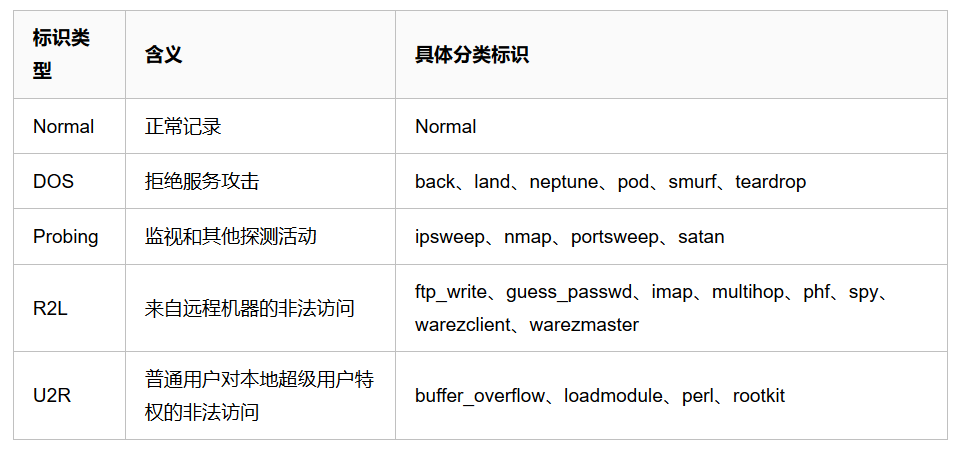
\includegraphics[width=0.98\textwidth]{fig_03_01.png}
	\caption{训练数据集标识类型}
	\label{}
\end{figure}
数据特征:KDD99训练数据集中有42维特征,其中前41维特征是连接记录的固定特征,最后一维是类标识符,用于指示连接记录是正常还是特定攻击类型。 在前41维特征中,9个特征属性是离散的数据,而其他属性是连续的数据。如下图3-2所示。

\begin{figure}[h]
	\centering
	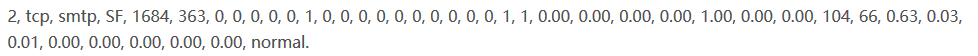
\includegraphics[width=0.98\textwidth]{fig_03_02.png}
	\caption{KDD99训练数据集}
	\label{}
\end{figure}

\subsection{数据预处理}
\subsubsection{观察数据}
\subsubsection{离散型数据预处理}
离散数据,也称字符型数据。计算机不能直接处理字符型数据,因此我们需要在算法开始之前对数据进行一系列的特征处理、转换。

针对KDD99数据集中的四类字符型数据做如下处理:

\subsubsection{连续型数据预处理}
	\begin{enumerate}  
		\item 设置变量X为数据集,变量Y为标签:
			
			\begin{figure}[h]  % [h]排版时把图片放在当前位置  浮动体就放在当前页面上,适合小浮动体
				\centering
				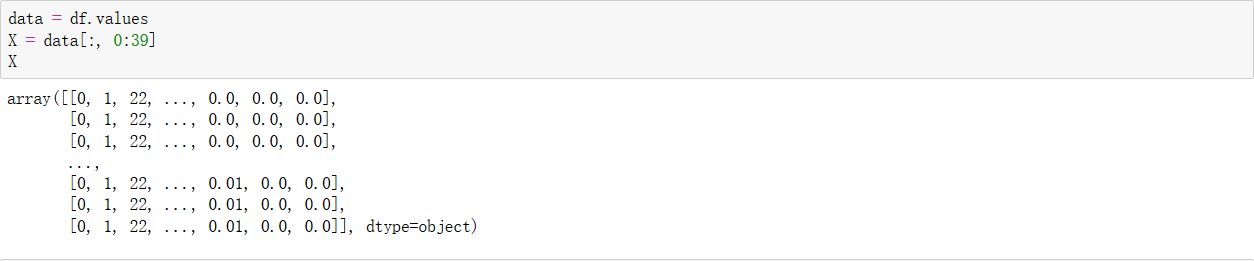
\includegraphics[width=0.98\textwidth]{fig_03_17.png}
				\caption{数据集X}
				\label{}
			\end{figure}
			\begin{figure}[h]  % [h]排版时把图片放在当前位置
				\centering
				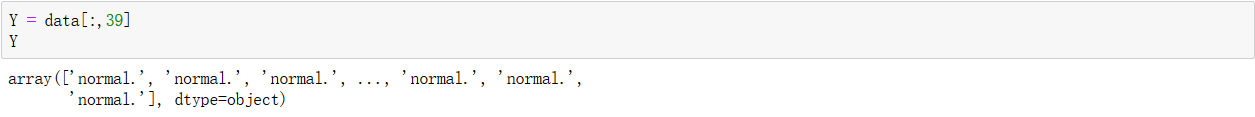
\includegraphics[width=0.98\textwidth]{fig_03_18.png}
				\caption{数据集Y}
				\label{}
			\end{figure}
		\item 设置变量X为数据集,变量Y为标签:
			
			进行数据标准化的原因:对于同一个特征来说,不同的样本中的取值有可能会相差很常大,一些异常的数据会误导模型的正确训练;除此之外,如果数据的分布很分散也会影响训练结果。以上两种数据的数据方差会非常大。此时,我们可以将特征中的值进行标准差标准化,即转换为均值为0,方差为1的正态分布。
	
			其原理是 
			$$x^{*}=\frac{x-\overline{x}}{\sigma}$$  % 单独占一行,mathpix
			其中,$x^*$为原始数据的均值,$\sigma$为原始数据的标准差。$\sigma$反应了给定数据距离其均值标准差的大小,高于平均值的数据将获得正标准化分数,反之亦然将获得负标准化分数。
			
			本实验使用python中的sklearn.preprocessing.StandardScaler类,通过
			StandardScaler模块计算标准化。标准化数据如下:
			\begin{figure}[h]  % [h]排版时把图片放在当前位置
				\centering
				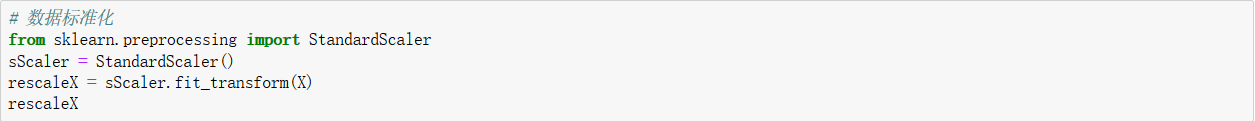
\includegraphics[width=0.98\textwidth]{fig_03_19.png}
				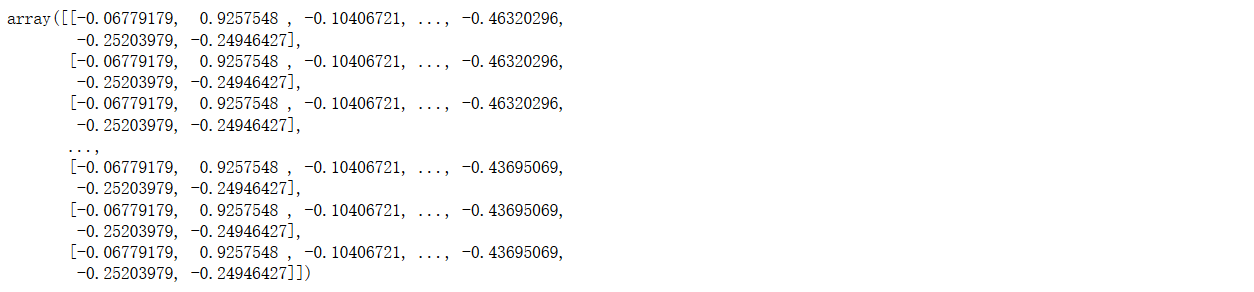
\includegraphics[width=0.98\textwidth]{fig_03_19_2.png}
				\caption{标准化后的数据}
				\label{}
			\end{figure}

		\item 对数据进行归一化:
		
			进行数据归一化的原因:拿到数据样本时,数据的单位往往不一致,在计算期间将数据缩放到特定间隔。处理用于比较和评估的指标时,可以将数据的单位限制去除并且将其转换为无量纲值,从而比较和加权不同单位或大小的指标。


	\end{enumerate} 

	 
	


\subsubsection{特征降维}
\begin{figure}[h]  % [h]排版时把图片放在当前位置
	\centering
	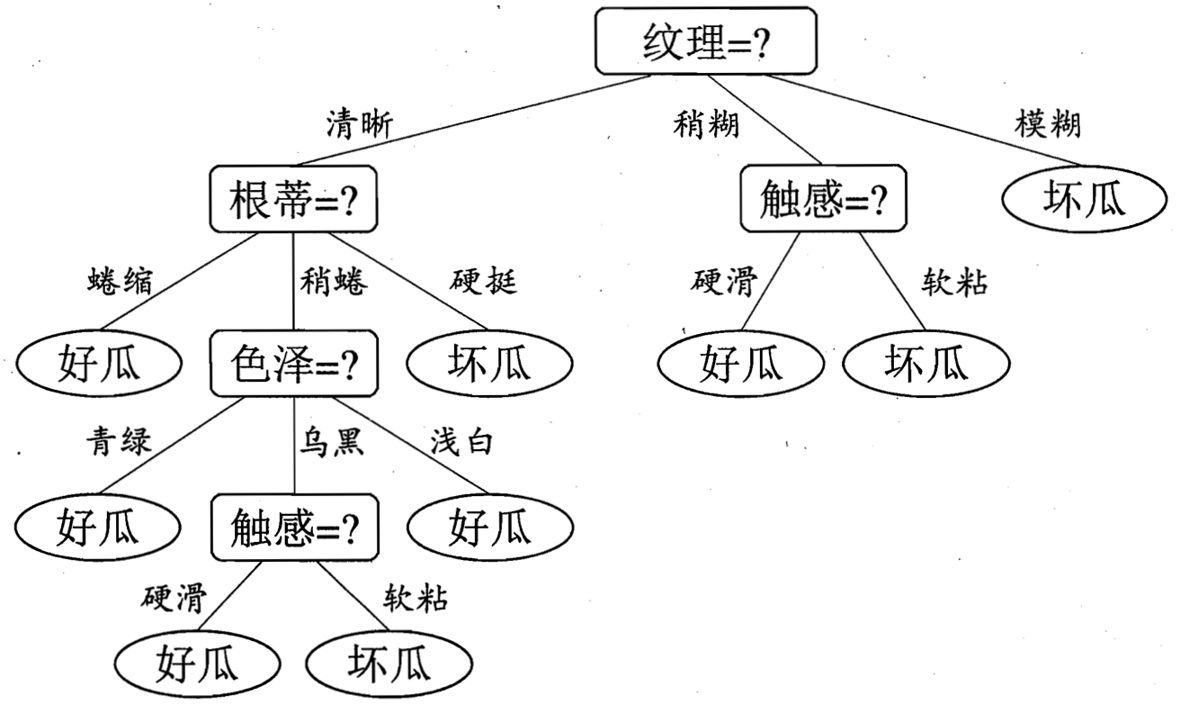
\includegraphics[width=0.98\textwidth]{fig_03_22.jpg}
	\caption{西瓜书}
	%\label{fig:1} % label放在caption之后,格式:书签名:类型:类名
	\label{}
\end{figure}

西瓜书 \footnote{周志华,《机器学习》}中写道:
\begin{quotation}
{\kaishu 归纳(induction)和演绎(deduction)是科学推理的两大基本手段,归纳是从特殊到一般的“泛化”(generation)的过程}	
\end{quotation}



\subsection{本章小结}
总结一下。

\setcounter{table}{0}  % 表格编号置0
\setcounter{figure}{0} % 图片编号置0
\setcounter{equation}{0} % 方程号置0 % 章节3
\section{基于聚类算法的入侵检测研究}

\subsection{k-means算法介绍}
k-means算法是一种简单的划分聚类算法,它通过计算样本之间的距离大小将样本集划分为k个簇。聚类目标是使同一个簇中的相关对象尽可能相互“接近”,而不同簇中的对象尽可能地“远离”。

\IncMargin{1em} % 使得行号不向外突出 
\begin{algorithm} 
	\caption{kmeans}
	\label{algo:1} 
	\KwData{样本数据集 $D$, 聚类簇数 $k$} 
	\KwResult{聚类集合} 
	$r\leftarrow t$\; $\Delta B^{\ast}\leftarrow -\infty$\; \While{$\Delta B\leq \Delta B^{\ast}$ and $r\leq T$}{$Q\leftarrow\arg\max_{Q\geq 0}\Delta B^{Q}_{t,r}(I_{t-1},B_{t-1})$\; $\Delta B\leftarrow \Delta B^{Q}_{t,r}(I_{t-1},B_{t-1})/(r-t+1)$\; \If{$\Delta B\geq \Delta B^{\ast}$}{$Q^{\ast}\leftarrow Q$\; $\Delta B^{\ast}\leftarrow \Delta B$\;} $r\leftarrow r+1$\;} 
\end{algorithm}
\DecMargin{1em}

从Algorithm \ref{algo:1}中可得 k-means 算法有以下缺点:
\begin{enumerate}  
	\item 聚类中心的k数量需要提前给出,但实际运用中,对于给定数据确定k值十分困难。很多时候我们不知道应该将这些数据集划分成几类最佳。
	\item k-means算法的聚类中心是随机选择的,选择不好的初始聚类中心,可能导致完全不同的聚类结果。
\end{enumerate}
\subsection{最佳k值选择}


\setcounter{table}{0}
\setcounter{figure}{0}
\setcounter{equation}{0} % 章节4
\section{总结} % 章节5
\newpage
\centerline{\zihao{3}{致\ \ \ \ 谢}}



\addcontentsline{toc}{section}{致\ \ 谢}

谢谢杨老师
 % 致谢

% 参考文献
\begin{thebibliography}{20}

\bibitem{Z-W1}
Zeng, Z., Wang, J.: Design and analysis of high-capacity associative memories based on a class of discrete-time
recurrent neural networks. IEEE Trans. Syst. Man Cybern., Part B, Cybern. 38(6), 1525–1536 (2008)

\bibitem{Z-W2}
Zeng, Z., Wang, J.: Design and analysis of high-capacity associative memories based on a class of discrete-time
recurrent neural networks. IEEE Trans. Syst. Man Cybern., Part B, Cybern. 38(6), 1525–1536 (2008)

\end{thebibliography}


% 附录
\centerline{\zihao{3}{附\ \ \ \ 录}}
\addcontentsline{toc}{section}{附\ \ 录}




\end{document}
